\documentclass[a4paper,11pt]{article}
\usepackage{fullpage}
\usepackage[latin1]{inputenc}
\usepackage[T1]{fontenc}
\usepackage[normalem]{ulem}
\usepackage[english]{babel}
\usepackage{listings,babel}
\lstset{breaklines=true,basicstyle=\ttfamily}
\usepackage{graphicx}
\usepackage{moreverb}
\usepackage{url}
\usepackage{amsmath}
\usepackage{float}
\usepackage{tabularx}

\title{Programmable Floating Point Unit}
\author{S\'ebastien Bourdeauducq}
\date{April 2010}
\begin{document}
\setlength{\parindent}{0pt}
\setlength{\parskip}{5pt}
\maketitle{}
\section{Overview}
The Programmable Floating Point Unit (PFPU) is a floating point VLIW microprocessor optimized for fast computation of vertices coordinates used by the Milkymist texture mapping unit.

It is designed for repetitive evaluation of the same mathematical function on a large number of points, using 32-bit floating point numbers. Furthermore, it contains specifically crafted DMA engine and address generator which enable the output DMA buffer to be ready to be used immediately by the texture mapping unit.

\section{Architecture}

\begin{figure}[H]
\centering
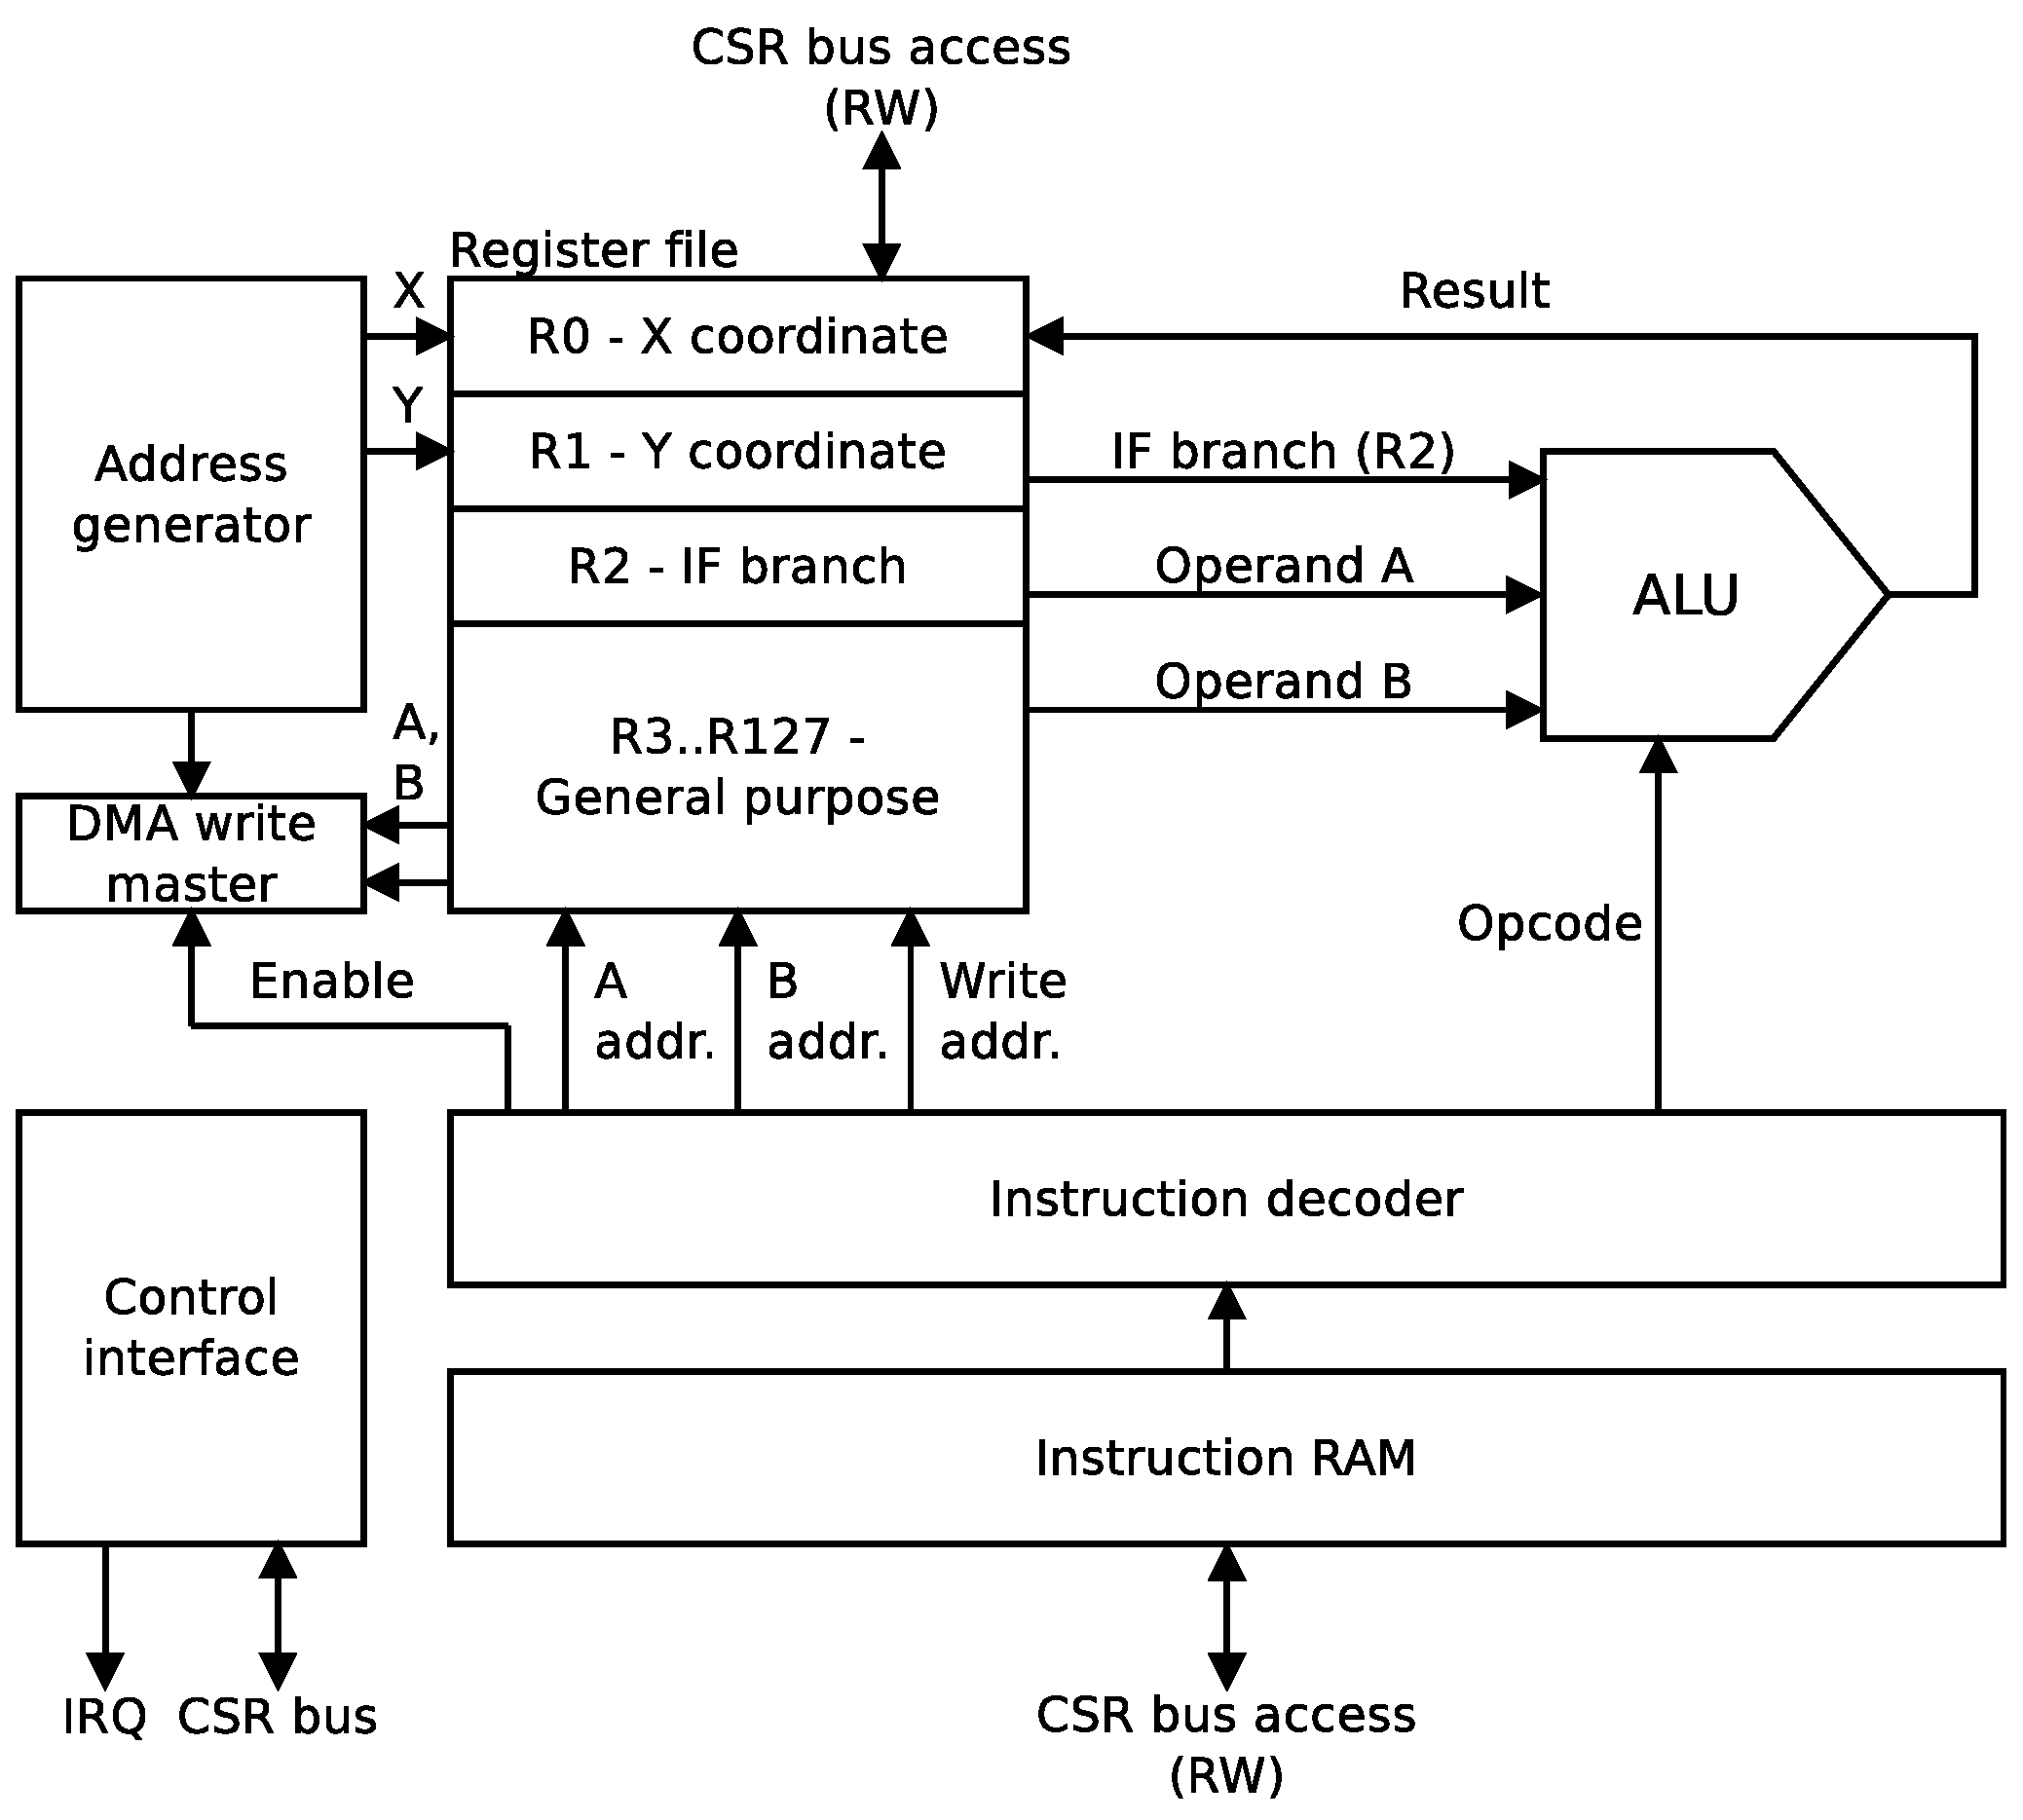
\includegraphics[height=100mm]{architecture.eps}
\caption{The PFPU architecture.}\label{fig:architecture}
\end{figure}

\subsection{Register file}
The PFPU implements 128 registers, which are accessed by its microcode, the address generator and the CSR interface.\\

\begin{tabularx}{\textwidth}{|l|l|l|l|X|}
\hline
\bf Register & \multicolumn{3}{|c|}{\bf Access} & \bf Description \\
\hline
 & \bf Ucode & \bf Addr. gen. & \bf CSR & \\
\hline
R0 & R & W & -- & Mesh X coordinate of the currently computed point, stored as integer by the address generator before starting the microcode. \\
\hline
R1 & R & W & -- & Mesh Y coordinate of the currently computed point (same remark). \\
\hline
R2 & RW & -- & RW & Selects the branch to return when executing an IF instruction. \\
\hline
R3--R127 & RW & -- & RW & General purpose 32-bit registers. \\
\hline
\end{tabularx}\\

The compiler can use the general purpose registers to store inputs of the function to be evaluated, and to store intermediate computation results.

The registers are not reinitialized when a new point is computed. It is the responsibility of the compiler to generate a microcode that does not overwrite inputs that must be used to compute several points.

Microcode writes to read-only registers result in undefined behaviour.

\subsection{Instruction set}
The microcode is specified a simple 25-bit instruction set. All instruction scheduling is handled by the compiler. \\

On each cycle, the PFPU executes two instructions, a read + start operation instruction that pushes two registers into the ALU, and a write instruction that takes the current ALU result and writes it back to the register file. The two are encoded in the same insctruction word. \\

\begin{tabular}{|l|l|l|l|l|}
\hline
\bf Parameter & Operand A & Operand B &  Opcode & Destination \\
\hline
\bf Length & 7 & 7 & 4 & 7 \\
\hline
\bf Bits & \verb!24..18! & \verb!17..11! & \verb!10..7! & \verb!7..0! \\
\hline
\end{tabular}\\

All instructions that do not write to the register file must have the ``destination'' field set to 0.

\subsection{Address generator}
The address generator iterates over all the points of a rectangular mesh. At each point, the ``X coordinate'' and ``Y coordinate'' registers are updated, and the DMA target address is computed.

The function used to compute the DMA target address is the same as the one of the texture mapping unit:

\begin{equation*}
base + 8 \cdot (128 \cdot y + x)
\end{equation*}

\subsection{Arithmetic and logical unit (ALU)}
The ALU contains several computation units that perform arithmetic, binary and logic operations.

At every cycle, a computation unit is selected using the ``opcode'' part of the instuction, according to the table below. The computation unit finishes its computation a number of cycles later, and the result is written to the register given in the instruction which is active at this time. It is the responsibility of the compiler to avoid output conflicts; that is to say, that only one unit may finish its computation at a given cycle.

Units can accept a new operation at each cycle (they are pipelines).

Each computation unit can have one, two or three arguments. If the unit has one argument, operand A is used, and operand B and flags are ignored. If the unit has two arguments, operands A and B are used. If the unit has three arguments, all operands and flags are used.

\subsubsection{Table of operations}

\begin{tabularx}{\textwidth}{|l|l|l|l|X|}
\hline
\bf Mnemonic & \bf Opcode & \bf Latency & \bf Description \\
\hline
NOP & 0 & -- & No operation (use as filler). \\
\hline
FADD & 1 & 4 & Floating point addition. \\
\hline
FSUB & 2 & 4 & Floating point subtraction (A-B). \\
\hline
FMUL & 3 & 5 & Floating point multiplication. \\
\hline
FABS & 2 & 2 & Floating point absolute value. \\
\hline
F2I & 5 & 2 & Convert float to integer. \\
\hline
I2F & 6 & 3 & Convert integer to float. \\
\hline
VECTOUT & 7 & -- & Write 2x32-bit vector to memory and terminate program. \\
\hline
SIN & 8 & 4 & Sine table look-up. \\
\hline
COS & 9 & 4 & Cosine table look-up. \\
\hline
ABOVE & a & 2 & Result is 1.0 is A>B, 0.0 otherwise. \\
\hline
EQUAL & b & 2 & Result is 1.0 is A=B, 0.0 otherwise. \\
\hline
COPY & c & 2 & Result is A. \\
\hline
IF & d & 2 & Result is A if R2 != 0, B otherwise. \\
\hline
TSIGN & e & 2 & Inverts the sign of A if B is negative. \\
\hline
QUAKE & f & 2 & Returns an inverse square root approximation. \\
\hline
\end{tabularx}\\

\subsubsection{Relationship with IEEE754}
When using floating point numbers, the PFPU uses the same number representation as IEEE754 (1-bit sign, 8-bit biased exponent, 23-bit mantissa). This is made to ease interfacing with IEEE754-compliant systems and software; however, the PFPU does not comply with IEEE754 and notoriously differs from the norm in the following points:

\paragraph{Denormal numbers.} The PFPU represents zero as any number that has a zero biased exponent, and the other bits are don't care. This means that denormal numbers are treated as zero. Therefore, when writing a floating point number to the PFPU, no special care should be taken to check if it's denormal or not (except for the obvious loss of precision). However, when reading a floating point number from the PFPU, if its exponent is zero, then its other bits are invalid. They must be ignored unless your use of the number can tolerate the introduced noise.

\paragraph{Precision.} The PFPU does not follow IEEE754 specifications regarding precision and rounding of operations.

\paragraph{Special numbers.} Numbers like NaN, infinity, etc. are not supported. Trying to perform an operation that would result in such a number in IEEE754-compliant arithmetics yields undefined result on the PFPU.

\subsubsection{Floating point addition and subtraction}
These operations are implemented using the same pipeline.

The operation is performed using one guard digit and truncation of the result.

\subsubsection{Integer conversions}
The PFPU supports conversion to and from 32-bit signed integers, using two's complement. When doing a float to integer conversion, the decimal part is truncated.

\subsubsection{Vector output}
This instruction takes two 32-bit integers A and B as input, and writes them in order to memory (A is written first). It formats the output of the PFPU so that it can be directly read as a vertex coordinate by the texture mapping unit.

Executing this instruction terminates the PFPU program.

\subsubsection{Sine and cosine table look-up}
This computes $sin(\frac{2 \cdot \pi \cdot A}{8192})$ or $cos(\frac{2 \cdot \pi \cdot A}{8192})$ for a signed integer input A. A can be of the whole 32-bit signed integer range ($-2^{31}$ to $2^{31}-1$) and the result will be correct, which makes preliminary range reduction to $[0;2\cdot\pi]$ unnecessary in practical cases. To compute sine or cosine, all you would need to do is a floating point multiplication by $\frac{8192}{2 \cdot \pi}$, conversion to integer, and sine/cosine table look-up.

\subsubsection{Comparison}
The \verb!ABOVE! and \verb!EQUAL! operations return a floating point number which is 0.0 (false) or 1.0 (true), depending on the result of the comparison.

\subsubsection{QUAKE instruction}
This instruction returns \verb!0x5f3759df - ((A & 0x7fffffff) >> 1)!. It is used to compute an approximation of the inverse square root, according to the algorithm made famous by Quake III.

\section{Interface}
The PFPU is equipped with a CSR slave bus used for control, and a Wishbone master for storing the computation results into system memory.

The CSR bus gives access to configuration and status registers, to the contents of the 128 data registers, and to the microcode memory.

\subsection{Register 0x000 -- Control register}
\begin{tabularx}{\textwidth}{|l|l|l|X|}
\hline
\bf Bits & \bf Access & \bf Default & \bf Description \\
\hline
0 & RW & 0 & Start/busy bit. Writing 1 to this position starts the execution of the microcode. When reading, this bit is set when the core is busy. \\
\hline
31--1 & --- & 0 & Reserved. \\
\hline
\end{tabularx}

\subsection{Register 0x004 -- DMA base register}
This register sets the base address for DMA transfers, expressed in bytes. DMA transfers must be aligned to a 32-bit boundary.

When the PFPU is busy (microcode execution in progress), this register is read-only. Writing it results in undefined behaviour.

\subsection{Registers 0x008 and 0x00C -- Last vertex index registers}
These registers set the indices of the last vertices of the mesh, respectively horizontally and vertically. Indices start at 0. For instance, when computing a mesh of 32x24 vertices, the registers should be set to 31 and 23.

When the PFPU is busy, these registers are read-only.

\subsection{Register 0x010 -- Microcode page register}
Because the CSR address space is limited, the 2048-word microcode memory is split into 4 consecutive pages of 512 words, and only one of these pages is mapped to the CSR interface at a given time. This register selects which. Values are between 0 to 3.

\subsection{Register 0x014 -- Vertex counter register}
This register counts the number of processed vertices. It can be read at any time, including when the core is busy. It is set to 0 when a new computation is started.

\subsection{Register 0x018 -- Collision counter register}
This register counts the number of \textit{collisions} that occured. A \textit{collision} happens when two pipelines finish their computations in the same clock cycle - and the microcode must be made so that this situation is avoided. The counter is set to 0 when a new computation is started.

\subsection{Register 0x01C -- Stray write counter register}
This register counts the number of \textit{stray writes} that occured. A \textit{stray write} happens when a pipeline finishes a computation, but the microcode defines no destination register for it. The counter is set to 0 when a new computation is started.

For stray write detection to work, all unused destination register slots in the microcode must be set to 0.

\subsection{Registers 0x400 to 0x5FC -- Register file access}
This address range gives direct access to the 128 registers of the file.

It should not be accessed while the microcode is in execution.

\subsection{Registers 0x800 to 0xFFC -- Microcode access}
This address range gives direct access to a page of 512 words of the microcode. The 25-bit microcode words are padded to 32 bits by adding 7 zeros before them.

It should not be accessed while the microcode is in execution.

\section{Interrupts}
The PFPU is equipped with one active-high edge-sensitive interrupt line.

An interrupt is triggered when a microcode has finished execution and all resulting data has been sent through the bus master.

\section*{Copyright notice}
Copyright \copyright 2007-2010 S\'ebastien Bourdeauducq. \\
Permission is granted to copy, distribute and/or modify this document under the terms of the GNU Free Documentation License, Version 1.3; with no Invariant Sections, no Front-Cover Texts, and no Back-Cover Texts. A copy of the license is included in the LICENSE.FDL file at the root of the Milkymist source distribution.

\end{document}
